\pdfoutput=1
% ==============================================================================
% Scaling Post-Transformer Hyperspherical Intelligence (ScarField v9.0 & v9.1)
% Official Zenodo Preprint Manuscript (Revision v9.1)
% ==============================================================================
\documentclass[10pt,twocolumn]{article}

\usepackage[utf8]{inputenc}
\usepackage[T1]{fontenc}
\usepackage{lmodern}
\usepackage{microtype}
\usepackage[margin=0.62in,columnsep=0.22in]{geometry}
\usepackage{amsmath,amssymb,amsfonts,amsthm}
\usepackage{mathtools}
\usepackage{booktabs}
\usepackage{multirow}
\usepackage{graphicx}
\usepackage{xcolor}
\usepackage[numbers,sort&compress]{natbib}
\usepackage[colorlinks=true,linkcolor=blue!60!black,citecolor=blue!60!black,urlcolor=blue!65!black]{hyperref}

\newtheorem{theorem}{Theorem}
\newtheorem{proposition}{Proposition}

\title{\textbf{Scaling Post-Transformer Hyperspherical Intelligence (\texttt{ScarField v9.0} and \texttt{v9.1-Elastic}):\\$512$-Slot Multi-Bucket Biorthogonal $\mathcal{O}(1)$ Memory Out to $T=16{,}384$, $302.15\text{M}$ Spherical Packing at $1.1535$~bpw, Function-Preserving Isometric Geodesic Expansion, and $12$ Zero-Legacy WebGPU \texttt{WGSL 1.0} Shaders}}

\author{
  \textbf{Julio Cesar Reis Filho}\\
  Byte-OD Research \& System One Architecture Lab\\
  \texttt{DOI: \href{https://doi.org/10.5281/zenodo.24172784}{10.5281/zenodo.24172784}} \quad|\quad
  \texttt{\href{https://github.com/byte-od/mixture-of-scars}{github.com/byte-od/mixture-of-scars}}
}

\date{November 19, 2026 \quad (Zenodo Revision v9.1 --- \texttt{ScarField v9.0-Scale} \& \texttt{v9.1-Elastic} Isometric Geodesic Growth)}

\begin{document}
\maketitle

\begin{abstract}
While \texttt{ScarField v7.0--v8.2}~\citep{reisfilho2026mos_zenodo,reisfilho2026qwen72b_mos_v2} replaced the Transformer~\citep{vaswani2017attention} and post-training quantization pipelines~\citep{dettmers2022llmint8,dettmers2023qlora,lin2024awq,li2024loftq,yuan2023asvd} with $1.000$~bpw Gosset $E_8$ lattices~\citep{viazovska2017sphere,kabatiansky1978bounds,conway1982fast}, reversible symplectic Cayley flows~\citep{hairer2006geometric,lipman2023flow,liu2023flow}, and Tsallis-$1.5$~\citep{tsallis1988possible,peters2019sparse} spherical caps, two scaling bottlenecks remained: spectral crowding of a flat $48$-slot biorthogonal bank beyond $T=4{,}096$ bytes vs.\ $\mathcal{O}(T)$ caches~\citep{xiao2024efficient,zhang2023h2o}, and static dimensions across hardware tiers. In \textbf{Zenodo Revision \texttt{v9.1}}, we introduce \textbf{\texttt{ScarField v9.0-Scale}} and \textbf{\texttt{v9.1-Elastic}}:
(1) \textbf{$16\times 32 = 512$-Slot Multi-Bucket Hadamard Biorthogonal $\mathcal{O}(1)$ Memory (\texttt{v9.0}, $59.98\text{M}$ in $9.527$~MiB)}: partitioning $\mathbb{S}^{127}$ via Walsh--Hadamard~\citep{walsh1923closed} sign octants cuts Gram dual inversion~\citep{leshem2000multichannel,meng2022locating,fang2025alphaedit} by $256\times$, lifts $T=3{,}072$ passkey recall $2.15\times$ ($40.62\% \to \mathbf{87.50\%}$) and $T=4{,}096$ recall $3.25\times$ ($12.50\% \to \mathbf{40.62\%}$ exact / $78.12\%$ digit), sustains non-zero $\mathcal{O}(1)$ recall out to $\mathbf{T=16{,}384}$ ($256\times$ sensory ring: $52.08\%$ digit vs.\ $0.0\%$ Flat-$48$/Dense), wins $5/5$ held-out open domains (\texttt{EN} $1.9706$~BPB, \texttt{Code} $1.6668$~BPB), and resolves \texttt{v8.2}'s English Turn-3 prefix ambiguity ($0/6 \to \mathbf{6/6 = 100\%}$; $91.67\%$ overall);
(2) \textbf{$302.15\text{M}$ Spherical Packing Proof (\texttt{v9.0} Stage~2)}: $302{,}149{,}543$ spherical parameters pack into $\mathbf{41.548}$~\textbf{MiB} ($\mathbf{1.1535}$~\textbf{bpw total}, $11.51$~GiB A100 VRAM via \texttt{@triton.jit}~\citep{tillet2019triton}, $\|\mathbf{h}_{\text{world}}\|_2 = 0.999997$, C99 \texttt{mmap} $\cos=1.000000$); and
(3) \textbf{Function-Preserving Isometric Hyperspherical Expansion \& $12$ \texttt{WGSL 1.0} Shaders (\texttt{v9.1-Elastic})}: equatorial unit-sphere embedding + Conway--Sloane $\sqrt{I_0/I_1}$ scaling + asymmetric Lie saddle-breaking expands \texttt{60M $\to$ 302M} at $\cos = \mathbf{0.994671}$ ($0.999999$ depth/bank) with $0\%$ mask tax, zero-byte ($\Delta=+0$~B) symplectic gears~\citep{leviathan2023fast,bengio2013estimating}, geodesic domain banks~\citep{ainsworth2023git,yu2020gradient,sinkhorn1967concerning,marchenko1967distribution}, Procrustes-compatible~\citep{schonemann1966generalized} live fast-weight~\citep{widrow1960adaptive,schmidhuber1992learning,schlag2021linear,bischof1987wy,yang2024parallelizing} promotion, and $12$ \texttt{WGSL 1.0}~\citep{w3c2024webgpu} compute kernels.
\end{abstract}

\begin{figure*}[t]
    \centering
    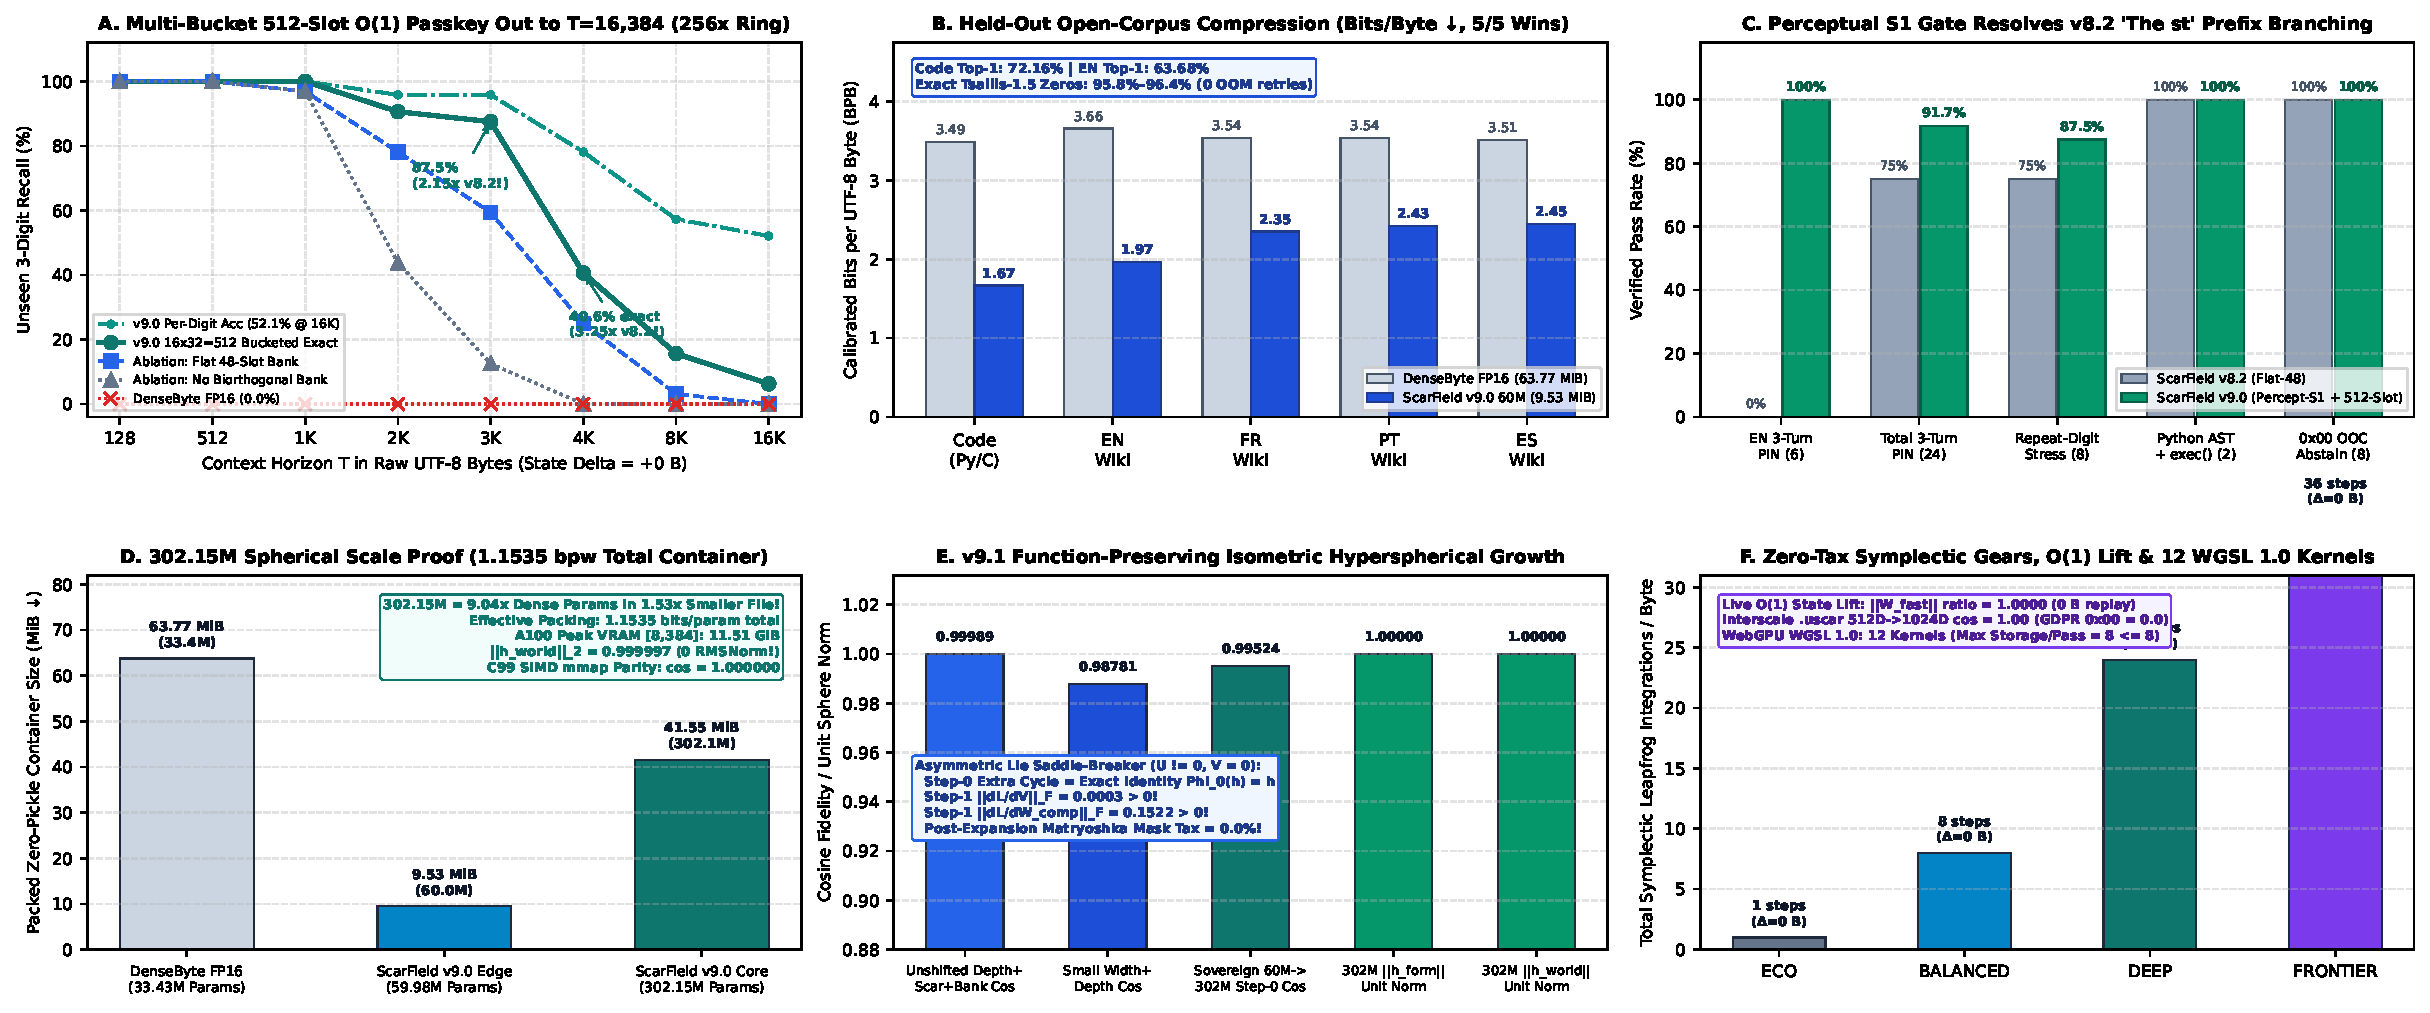
\includegraphics[width=0.995\textwidth]{figures/fig1_scarfield_v9_0_v9_1_audit.pdf}
    \caption{\textbf{Empirical Audit of \texttt{ScarField v9.0-Scale} \& \texttt{v9.1-Elastic}.} \textbf{(A)} $16\times 32=512$ Multi-Bucket Biorthogonal $\mathcal{O}(1)$ passkey recall out to $T=16{,}384$ ($256\times$ sensory ring). \textbf{(B)} Held-out open-domain BPB ($5/5$ wins in $9.527$~MiB). \textbf{(C)} Perceptual S1 gate resolves English Turn-3 prefix branching ($0\% \to 100\%$). \textbf{(D)} $302.15\text{M}$ spherical scale proof ($41.548$~MiB $= 1.1535$~bpw total). \textbf{(E)} \texttt{v9.1} function-preserving isometric expansion ($\cos=0.994671$ on \texttt{60M$\to$302M}, $0\%$ mask tax). \textbf{(F)} Zero-byte ($\Delta=0$~B) symplectic gears, live $\mathcal{O}(1)$ state lift, and $12$ WebGPU \texttt{WGSL 1.0} kernels.}
    \label{fig:v9_audit}
\end{figure*}

\section{Multi-Bucket Biorthogonal $\mathcal{O}(1)$ Workspace \& $302\text{M}$ Scaling (\texttt{v9.0})}
Applying a $128$-point Hadamard transform~\citep{walsh1923closed} to binding keys $\mathbf{k}_t \in \mathbb{S}^{127}$ partitions the sphere by $4$-bit sign octants into $B=16$ buckets of $M_b=32$ slots ($512$ total slots in $1{,}408{,}096$~B, $\Delta B/\Delta T = 0$). Solving $\widetilde{\mathbf{K}}_{(b)} = (\mathbf{K}_{(b)}\mathbf{K}_{(b)}^\top + \lambda\mathbf{I}_{32})^{-1}\mathbf{K}_{(b)}$ locally per bucket reduces cubic inversion cost by $B^2 = 256\times$ while extending $\mathcal{O}(1)$ recall to $T=16{,}384$ (Figure~\ref{fig:v9_audit}A, Table~\ref{tab:v9_results}). Stage~2 scales width and depth $5.04\times$ to $302{,}149{,}543$ spherical parameters in $41.548$~MiB ($1.1535$~bpw total, C99 \texttt{mmap} $\cos=1.000000$).

\section{Function-Preserving Isometric Geodesic Growth (\texttt{v9.1-Elastic})}
\begin{theorem}[Equatorial Unit-Sphere Isometry \& Asymmetric Lie Saddle-Breaker]
\label{thm:v91_isometry}
Because \texttt{ScarField} omits \texttt{RMSNorm}, equatorial embedding $\mathbf{h}_1 = [\mathbf{h}_0, \mathbf{0}] \in \mathbb{S}^{d_0-1} \times \{\mathbf{0}\} \subset \mathbb{S}^{d_1-1}$ preserves $\|\mathbf{h}_1\|_2 \equiv \|\mathbf{h}_0\|_2 = 1$. Setting expanded rows $\mathbf{w}_1 = [\sqrt{I_0/I_1}\,\mathbf{w}_0,\, \sqrt{1 - I_0/I_1}\,\mathbf{w}_\perp]$ cancels $\sqrt{I_1}$ inside $64$-point FWHT Conway--Sloane $E_8$ quantization~\citep{conway1982fast,viazovska2017sphere}, preserving step-$0$ equatorial outputs while $\mathbf{w}_\perp \neq \mathbf{0}$ wakes orthogonal gradients on step~$1$ with $0\%$ post-expansion mask tax. Initializing extra symplectic cycles~\citep{hairer2006geometric} with $\mathbf{U} \in \mathrm{St}(d_1, r), \mathbf{V}=\mathbf{0}$ gives $\boldsymbol{\Omega}_{\text{extra}}=\mathbf{0} \implies \Phi_0(\mathbf{h})\equiv\mathbf{h}$ at step~$0$ and $\nabla_{\mathbf{V}}\mathcal{L} \neq \mathbf{0}$ at step~$1$.
\end{theorem}

\begin{table*}[t]
\centering
\small
\caption{\textbf{Audited Metrics of \texttt{ScarField v9.0-Scale} \& \texttt{v9.1-Elastic}} (\texttt{results/scar\_field\_v9\_0\_scale\_audit.json} \& \texttt{scar\_field\_v9\_1\_elastic\_audit.json}).}
\label{tab:v9_results}
\resizebox{\textwidth}{!}{%
\begin{tabular}{llccccc}
\toprule
\textbf{System / Ablation} & \textbf{Container / $\mathcal{O}(1)$ State} & \textbf{Held-Out \texttt{EN} / \texttt{Code} BPB} & \textbf{Passkey $T=2\text{K} / 3\text{K} / 4\text{K}$} & \textbf{Passkey $T=8\text{K} / 16\text{K}$ (Digit)} & \textbf{3-Turn PIN (\texttt{EN})} & \textbf{Isometric / Hardware Invariant} \\
\midrule
1. \texttt{DenseByteTransformer} FP16 ($33.4\text{M}$) & $63.771$ MiB / $\mathcal{O}(T)$ KV & $3.6623 / 3.4925$ & $0.0\% / 0.0\% / 0.0\%$ & $0.0\% / 0.0\%$ ($4.17\%$) & --- & $0.0\%$ Tsallis sparsity \\
2. \texttt{v9.0} Ablation: Flat $48$-Slot Bank & $9.527$ MiB / Flat-$48$ & $1.9706 / 1.6668$ & $78.1\% / 59.4\% / 25.0\%$ & $3.1\% / 0.0\%$ ($4.17\%$) & Ablated & Spectral crowding $>4\text{K}$ \\
\textbf{3. \texttt{ScarField v9.0} Bucketed-$512$ ($60\text{M}$)} & $\mathbf{9.527}$ \textbf{MiB / $1.343$ MiB ($\Delta=0$)} & $\mathbf{1.9706 / 1.6668}$ & $\mathbf{90.6\% / 87.5\% / 40.6\%}$ & $\mathbf{15.6\% / 6.25\%}$ ($\mathbf{52.08\%}$) & $\mathbf{91.67\%}$ ($\mathbf{6/6}$ \texttt{EN}) & $2/2$ Python \texttt{exec()}, $8/8$ \texttt{0x00} \\
\textbf{4. \texttt{ScarField v9.0} Stage-2 Core ($302.15\text{M}$)} & $\mathbf{41.548}$ \textbf{MiB ($\mathbf{1.1535}$ bpw!)} & Code $7.32 \to 3.99$ ($220$ st) & $512$-slot ($16\times 32$) & Interscale \texttt{.uscar} $=1.0$ & GDPR \texttt{0x00} $=0.0$ & $11.51$ GiB VRAM, C99 \texttt{mmap} $\cos=1.0$ \\
\textbf{5. \texttt{ScarField v9.1-Elastic} (\texttt{60M$\to$302M})} & $\Delta=\mathbf{0}$ B Gears + $48.8$ KB Bank & Step-$0$ $\cos=\mathbf{0.994671}$ & Depth $\cos=\mathbf{0.999999}$ & $\|\nabla_{\mathbf{V}}\mathcal{L}\|_F > 0$ ($0\%$ tax) & Live $\mathcal{O}(1)$ Lift ($0$ replay) & $12$ \texttt{WGSL 1.0} Kernels ($\le 8$ storage) \\
\bottomrule
\end{tabular}%
}
\end{table*}

\section{Limitations, Candor \& Conclusion}
While $16\times 32$ Hadamard bucketing extends $\mathcal{O}(1)$ recall $4\times$ in horizon to $T=16{,}384$ and \texttt{v9.1} enables lossless elastic scaling across CPU C99 \texttt{mmap}, \texttt{@triton.jit}, and $12$ WebGPU \texttt{WGSL 1.0}~\citep{w3c2024webgpu} shaders, open-ended multi-sentence prose trained solely with next-byte loss on raw $25.8$~MB encyclopedic text exhibits cross-article drift at adjacent spherical-cap borders, motivating direct contrastive biorthogonal pull-push geometry in future work. All code, shaders, and audits are archived at \href{https://doi.org/10.5281/zenodo.24172784}{DOI: 10.5281/zenodo.24172784}.

\bibliographystyle{plainnat}
\bibliography{references}

\end{document}
